\chapter{System Application - Droplet Microluidics}
\section{Aims}
The application of the PDFC to droplet microfluidics serves two purposes. First, it verifies that the system is functioning as intended for use as a practical research tool. Second, it allows the characterization of droplet formation by a pressure driven flow in T-junction geometry, an area currently underdeveloped \cite{Christopher2008}. 

\section{Methods}
\subsection{Device Generation}

The T-junction microfluidic device referenced herein is fabricated using standard soft lithography methods \cite{Stroock2002}. Two part Polydimethylsiloxane (PDMS) was poured onto a SU-8 mold previously developed by Schmid and Franke \cite{Schmid2014c} to form an array of individual $25 \mu m \times 25 \mu m$ T-junction channels. The PDMS was cured at 65dC for 3 hours. After cooling to room temperature, the set PDMS was cut and removed from the mold. Tubing connection holes were punched using a standard $0.5mm$ biopsy punch. Next, both glass slide and the PDMS are oxygen-plasma treated, adhered, and exposed to 100dC for 1hour. Prior to use, devices are treated with the aquapel for 10mins, purged with filtered compressed gas and dried at 65dC for 3 hours. 

\subsection{Reagents}

Reagents were formulated in bulk, the same formulation was used for all data presented here. The continuous phase consists of 3M's HFE-7500 fluorocarbon oil stabilized with 2.0 wt\% fluorosurfactant ammonium carboxylate DuPont Krytox 157. This discontinuous phase consists of de-ionized water and Sigma Aldrich's B0126-256 Bromophenol blue, dissolved in 0.1M NaOH.

\subsection{Experimental Procedure}

The microfluidic device was installed on an upright microscope with 20X Objective and brightfield illumination. Images are acquired by Photon fastcam at 500 frames per second (fps). The applied control pressure was held constant for the continuous phase while varying the discontinuous phase control pressure to achieve varying flow conditions. Discontinuous phase control pressure was varied at intervals no smaller than $\approx$5mbar until droplet formation ceased due to the onset of backflow or instability, for low or high pressures, respectively. 

\subsection{Analysis of Collected Data}

The captured images were then analyzed using a custom imageJ script to determine droplet length, $L$, and position, $X$, along an arbitrarily defined axis parallel to the geometry's outlet channel.

\section{Results}
\label{sec:results}

\subsection{Regime Transition}

For the T-junction channel geometry described the dimensionless droplet ratio of droplet length, $L$, over channel width, $W$, is plotted as a function of the applied control pressure ratios, $\frac{P_{H_2O}}{P_Oil}$, shown in Figure \vref{fig:lwvpr}. Error bars have been calculated by standard deviation of measured droplet length which results in error equal to or smaller than the symbol size and thus not shown. Linear regression models have been applied to the data points expected to be within the squeezing regime. The slopes of the fitted line were determined as 3.909, 4.151, and 5.370 for applied continuous phase pressures of 40, 60, and 80 mbar with coefficients of determination of 0.958,0.996, 0.990, respectively. Full summary statics of the linear regression fit are presented in the Statistics Appendix.

\begin{figure}[H]
\centering 
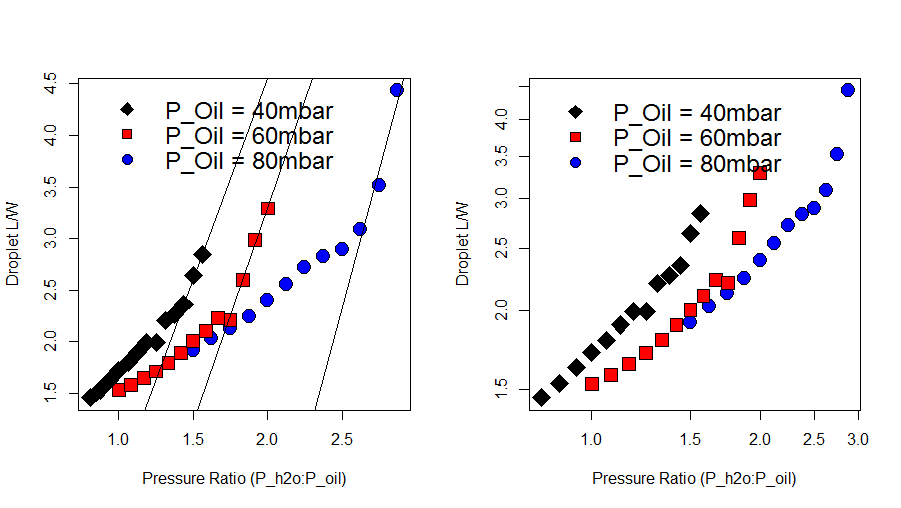
\includegraphics[width=01.0\columnwidth]{lwvpr.PNG} 
\caption[Droplet Length as a Function of Applied Control Pressure Ratio]{Log-log (left) and standard (right) plots of droplet length as a function of the applied control pressure ratio for T-junction geometry. Note the distinct change in slope as the pressure ratio increases.} 
\label{fig:lwvpr} 
\end{figure}

Outer Ca values are calculated given an interfacial tension of $\gamma = 2.87 \times 10^{-3}\frac{N}{m}$ (as measured by spinning method), continuous phase viscosity of $\mu = 1.24 \times 10^{-3} Pa \cdot s$\cite{3M2009}, and mean velocity, $u$, as determined by droplet position over consecutive frames.

Droplet length is plotted as a function of capillary number as shown in Figure \vref{fig:regimes2} for each of the applied continuous pressures. The critical capillary numbers were approximated as 0.0135, 0.0185, and 0.0215 for 40, 60 and 80 mbar continuous phase pressures, respectively. Images of droplet formation are shown within the squeezing and dripping regimes for each continuous phase control pressure. The images shown are captured one frame prior to droplet formation. 

\begin{figure}[H]
\centering 
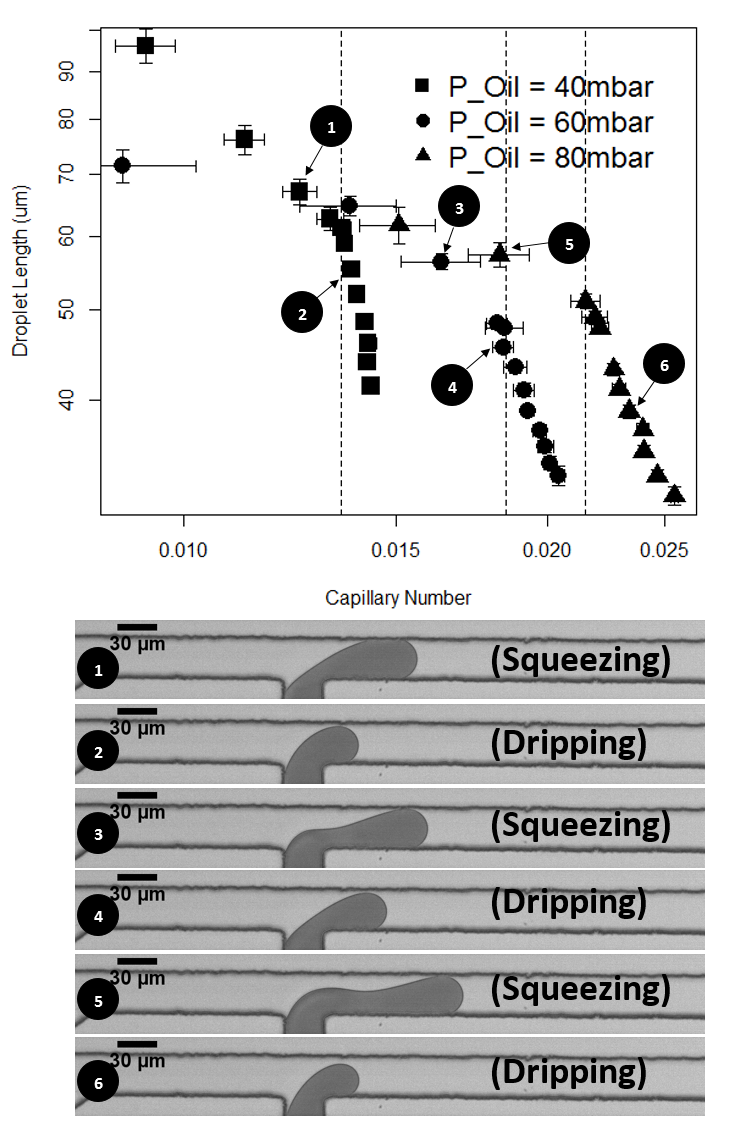
\includegraphics[width=0.75\columnwidth]{regimes2.PNG} 
\caption[Droplet length as a function of Capillary number across squeezing and dripping regimes]{Top: Droplet length as a function of Capillary number across squeezing and dripping regimes. The transition between dripping and squeezing regimes is marked by vertical dashed lines, corresponding to critical capillary numbers of 0.0135, 0.0185, and 0.0215. Bottom: Typical images of droplet elongation just prior to formation.} 
\label{fig:regimes2} 
\end{figure}

\clearpage

\subsection{Droplet Polydispersity}

Variance in droplet dimensions is analyzed by evaluating the length of droplets formed by constant applied control pressures. Images were acquired at 500 fps for a period of 10 seconds resulting in a sample size of at least 100 droplets with at least three length measurements taken in subsequent frames per unique droplet. A variety of plots investigating population statistics are shown in Figure \vref{fig:1_poly}, for data acquired at $P_{OIL} = 20mbar,  P_{H_2O} = 80mbar$, resulting in a $Ca$ value of 0.010. The same analysis was conducted at two higher $Ca$ values and is found in Statistics Appendix .

\begin{figure}[H]
\centering 
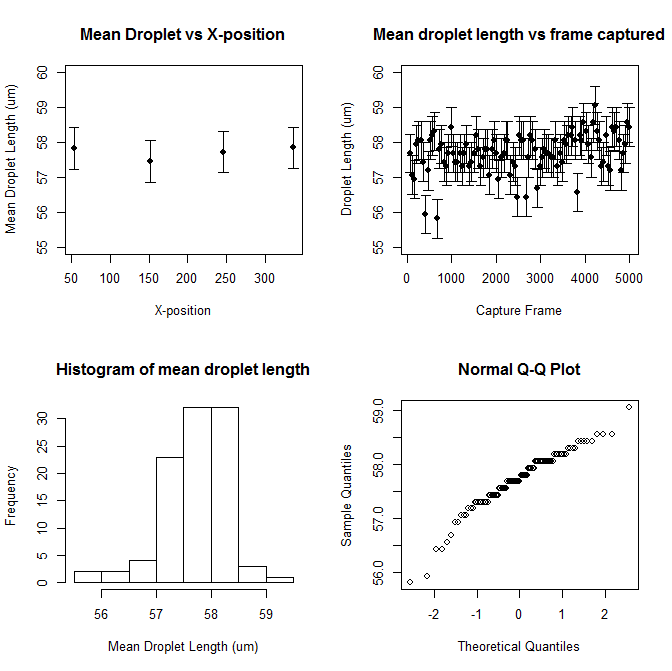
\includegraphics[width=01.0\columnwidth]{1_poly.PNG} 
\caption[Polydispersity]{Population distribution of droplet length for $P_{oil} = 0.1 bar, Ca = 0.010$. Top-left: Mean droplet length as shown by measured X-position. Top-right: Droplet length shown over the duration of image acquisition. Bottom-left: Histogram of measured droplet length. Bottom-right: Q-Q plot for the droplet length population.} 
\label{fig:1_poly} 
\end{figure}

\clearpage

From the analyzed data, droplet velocity, flowrate, capillary number, mean length, length standard deviation and percent Coefficient of Variation are extracted. A summary of the resulting dimensional statistics is shown in Table \vref{tab:poly}.

\qquad

\begin{table}[H]
\begin{tabular}{l*{6}{c}r}
$ P_{Ratio} $ & $ V_C  (m/s) $ &  $ Q_C ( \mu  L/min) $ & Ca & $ Mean Length( \mu m )$ & $ StdDev( \mu m) $ & C.V. \\
\hline
4 & 0.023 & 0.863 & 0.010 & 57.71 & 0.55 & 0.95 \\
2.25 & 0.033 & 1.238 & 0.014 & 54.53 & 0.35 &  0.64 \\
1.66 & 0.043 & 1.613 & 0.018 & 48.14 & 0.21 &  0.43 \\
\end{tabular}
\caption[Droplet Polydispersity]{Dimensional analysis of droplets}
\label{tab:poly} 
\end{table}


\clearpage


\section{Discussion}
\subsection{Droplet Regime Transition}

Previous work has been done to establish specific flow regimes in which droplets are formed in T-junction geometry by both numeric modeling and experimental investigations \cite{Abate2012a},\cite{DeMenech2008},\cite{Garstecki2006}. Previous findings suggest that two stable droplet formation regimes exist in T-junction droplet formation, \emph{dripping} and \emph{squeezing}. In a highly cited paper, De Menech et al showed by numerical modeling that the transition between the two distinct droplet regimes may be defined by a Critical Capillary Number, $Ca_{cr}$, and that this transition is independent of viscosity ratio and flowrates, shown in Figure \vref{fig:menechtransition} \cite{DeMenech2008}. 

This transition has been previously determined both experimentally and in numerical simulations to be $Ca_{cr}\approx 10^{-2}$. These values of Capillary Numbers represent a threshold below which the interfacial forces significantly dominate the viscous forces. Thus, in these geometries the discontinuous phase is only minimally elongated as it enters the T-junction and instead extends orthogonally to the main channels such that the channel is plugged prior to droplet formation. After the droplet blocks the channel outlet, break-up proceeds driven by the building pressure differential due to the blockage.

\begin{comment}
\begin{figure}[H]
\centering 
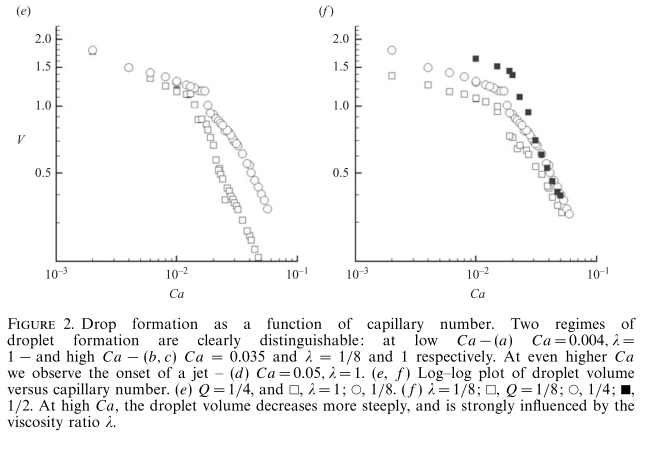
\includegraphics[width=0.75\columnwidth]{menechtransition.PNG} 
\caption[Menech Regime Transition]{Used directly, without permision} 
\label{fig:menechtransition} 
\end{figure}
\end{comment}

\emph{While the regime transition has been well documented through numerical simulations and in experiments utilizing volumetric-flow, to the best of the author's knowledge there has been no record of experimental observations demonstrating the regime transition from squeezing to dripping in a pressure-driven flow system.} This, despite the fact that there have been documented dissimilarities in volumetric versus pressure-driven flow in droplet formation\cite{Ward2005}, and that there may be advantages in droplet monodispersity in pressure-driven systems \cite{Christopher200,Li2014a}.

The data presented here shows a distinct transition between dripping and squeezing regimes, as demonstrated by the change in slope shown in Figure \vref{fig:lwvpr}. The plot shows a transition from dripping regime to squeezing regime as the pressure ratio increases. The squeezing regime appears to be linear as determined by the linear regression models. This linearity agrees with Gastecki's findings that within the squeezing regime droplet L/W is a function of only the channel geometry, represented by the $\alpha$ coefficient, and the  volumetric flowrates, $Q_{in} $and $ Q_{put}$ shown in Equation \vref{eq:garstecki} \cite{Garstecki2006}.

\begin{equation}
L/W = 1 + \alpha Q_{in} / Q_{out}
\label{eq:garstecki}
\end{equation}

Here, L/W data is presented as a function of applied pressure ratios rather than flowrate ratios and therefore cannot be directly compared. Furthermore, the data presented here exists precisely at the transitional capillary numbers and therefore contains droplets formed within both regimes as opposed to Garstecki's purely squeezing regime data. Therefore, in order to draw further conclusions regarding the application of the scaling law to the pressure-driven system both these complications must be overcome, as discussed further in the Conclusions Section.

The transition between regimes may also be shown by the changing behavior of droplet length as a function of capillary number shown in Figure \vref{fig:regimes2}. However, the $Ca_{cr}$ value at which the transition occurs is not universal between the different continuous phase pressures as shown previously \cite{DeMenech2008}. The transitional capillary number can be plotted as a function of the continuous phase pressure as shown in Figure \vref{fig:CrCaABline}.

\begin{figure}[H]
\centering 
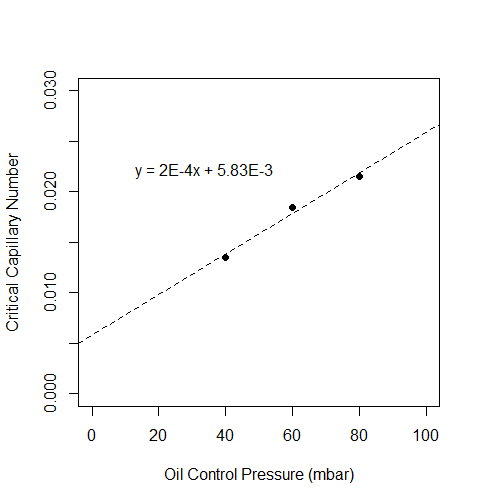
\includegraphics[width=0.75\columnwidth]{CrCaABline.PNG} 
\caption[Critical capillary number as a function of continuous phase applied pressure]{Critical capillary number as a function of continuous phase applied pressure} 
\label{fig:CrCaABline} 
\end{figure}

The difference in $Ca_{CR}$ is likely due to the use of droplet velocity as an approximation for mean continuous phase velocity. Others have expected that there is some numerical difference between the velocity of the droplets and the mean velocity of the continuous phase \cite{Ward2005}. Unfortunately, due to the complex nature of multiphase flow during droplet formation it may be difficult to further investigate the true mean velocity of the continuous phase. However, due to the linear nature of relationship between the applied control pressure of the continuous phase and the critical capillary number the velocities could be corrected such that the regime transition is coincident, as shown in Figure \vref{fig:ca_cor}. 

\begin{figure}[H]
\centering 
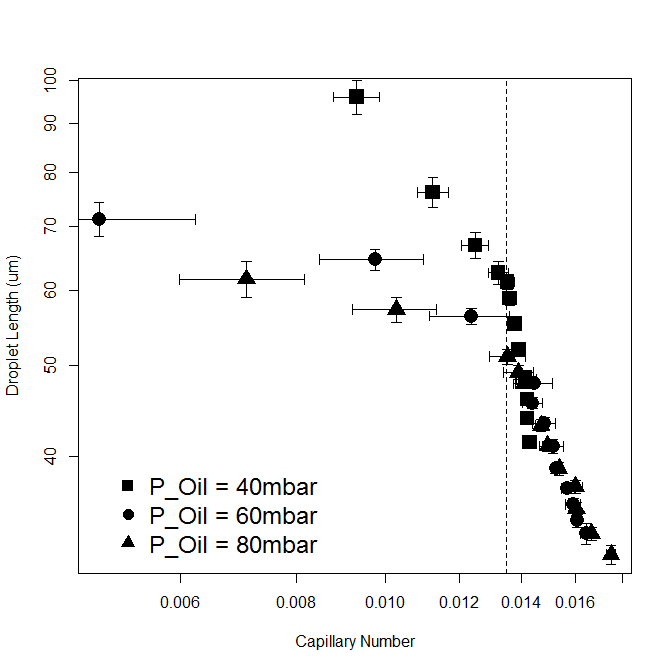
\includegraphics[width=0.750\columnwidth]{ca_cor.PNG} 
\caption[Droplet Length as a function of Corrected Capillary Number]{Droplet length as a function of corrected capillary number. The dashed vertical line shows the interpreted point of transition.} 
\label{fig:ca_cor} 
\end{figure}

This interpretation of the regime transition as a function of corrected critical capillary number is a simplification not without its own complications. Despite the critical capillary number appearing to be linearly related between the applied continuous phase pressures this does not appear to be the case for the entirety of the presented L vs. Ca curve.

One further point of discussion, highlighting the difference between volumetric and pressure-driven flows, is the existence of a quasi-equilibrium no flow condition. As the system is moved towards the lowest operational pressure ratios, the aqueous phase comes to a quasi equilibrium no-flow state, as previously reported by Ward et al \cite{Ward2005}. If the pressure ratio is decreased any further(either by increasing $P_{Oil}$ or decreasing $P_{H_2O}$) back-flow will occur, in which the continuous phase begins displacing the aqueous phase upstream towards the reservoir. This quasi equilibrium state may be described as a balance of forces between the pressure of the two phases and the Laplace pressure differential across the liquid-liquid interface, described as shown in Equation \vref{eq:noflow}.

\begin{equation}
P_{D_{Loc}} + P_{Laplace} = P_{C_{Loc}} 
\label{eq:noflow}
\end{equation}

Where Laplace pressure can be roughly approximated given $\gamma$ is the interfacial tension between the two phases, $r$ is the radius of curvature of the interface as \cite{Bruus2008}:
\begin{equation}
 P_{Laplace} = \frac{2 \gamma}{r}
\label{eq:laplace}
\end{equation}

It should be noted that here $P_{D_{Loc}}$ and $P_{C_{Loc}}$ represent the pressures of the two phases local to the T junction and that there is some unknown pressure drop between the applied control pressures at the inlet reservoirs and these local pressures. This pressure drop can be calculated using Hydraulic resistance as discussed in the Background Theory section.
 

\subsection{Droplet Polydispersity}

Polydispersity in syringe pump based systems suffers, particularly at low flow velocities, due to minor fluctuations in the stepper-motor-actuated syringe plungers\cite{Christopher2008}. Here, polydispersity is measured by the coefficient of variation (CV) on the population’s droplet length. In the populations measured, the CV was below 1\%. This is significantly lower than the 10\% CVs reported by experimental observations in T-junctions using syringe pumps at similar flowrates \cite{Christopher2008}. The results are similar to the polydisersity reported by others using pressure-driven flow. However, the CVs shown here suggest this system is capable of marginally improved monodispersity relative to the $~2\%$ CVs reported elsewhere and at even lower flowrates \cite{Lim2015, Kaminski2016}. The lowest continuous phase flowrate droplet population measured here was $0.863 \mu L / min$, resulting in a capillary number of $0.010$ and CV of $0.95$.

